\documentclass[a4paper, twocolumn, 9pt]{article}

% --- Essential Packages ---
\usepackage[utf8]{inputenc}
\usepackage[T1]{fontenc}
\usepackage{amsmath, amssymb}
\usepackage{graphicx}
\usepackage{booktabs}
\usepackage[columnsep=0.7cm, top=2cm, bottom=2cm, left=1.5cm, right=1.5cm]{geometry}
\usepackage{hyperref}

% --- Custom Math Commands ---
\newcommand{\dpo}{\text{DPO}}
\newcommand{\DPO}{\text{DPO}}

% --- Title Information ---
\title{\vspace{-1.5cm}\textbf{Steerability–Robustness Tradeoff in Language Models via Direct Preference Optimization ($\dpo$)}\vspace{0.5cm}}

\author{
    Mahmoud Zahran$^1$ \quad Yahya Al Malallah$^1$ \quad Kumail Alhamoud$^2$ \\
    \small $^1$King Abdullah University of Science and Technology (KAUST) \quad
    $^2$Massachusetts Institute of Technology (MIT) \\
    \small \texttt{mahmoud.zahran@kaust.edu.sa}, \texttt{yahya.almalallah@kaust.edu.sa}, \texttt{kumail@mit.edu}
}

\date{December 3, 2025}

% -------------------------------------------------------------
\begin{document}
\maketitle

% -------------------------------------------------------------
\begin{abstract}
Safety alignment aims to reduce harmful or unsafe behaviors in large language models (LLMs),
but is often assumed to impose a \emph{capability tax}: models become safer, but also less helpful
or overly cautious.
In this work we ask: \emph{can Direct Preference Optimization (DPO) achieve meaningful safety alignment
without degrading model capabilities?}
Using two open-weight model families---Llama 3.1-8B and Qwen 2.5-7B---we examine how preference-based
safety alignment affects both refusal behavior and general capabilities across five $\DPO$ configurations.

We construct a strictly filtered subset of PKU-SafeRLHF containing only unambiguous ``safe-vs-unsafe''
preference pairs and fine-tune models with LoRA adapters.
Safety is evaluated via refusal rates on AdvBench using GPT-4o as an LLM-as-judge,
and capabilities are measured on MMLU and GSM8K.

Across both model families we find that $\DPO$ substantially improves safety
(\(+60\) and \(+28\) percentage-point increases in refusal rate) while preserving---and in some cases improving---
capabilities: Llama gains \(+9.5\) MMLU points, and Qwen gains \(+2\) points.
Moderate-strength configurations yield the best tradeoff, but even aggressive alignment
does not catastrophically degrade performance.
Despite different pretrained safety baselines, both models can be steered into a high-safety, high-capability regime.
Our results demonstrate that with high-quality safety preferences, $\DPO$ can yield strong alignment \emph{without}
the severe capability tax often feared in practice.
\end{abstract}

% -------------------------------------------------------------
\section{Introduction}

Can we make language models safer without making
them dumber? As LLMs are deployed in increasingly
sensitive settings, this question sits at the heart of practical
alignment. Safety interventions such as supervised
safety fine-tuning, RLHF~\cite{rlhf}, and rule-based filters can re
duce harmful outputs, but practitioners frequently report
side effects: models over-refuse benign queries, hal
lucinate ``I cannot help with that'' in harmless contexts,
or lose performance on reasoning and knowledge benchmarks.
This has led to the prevailing concern that safety
alignment inevitably incurs a \emph{capability tax}.

Direct Preference Optimization ($\DPO$)~\cite{dpo} is a widely adopted
alignment method that sidesteps some of the complexity
of RLHF by directly optimizing over paired preference
data with a KL-regularized objective. DPO has been
used in many open-weight pipelines, often with
safety-oriented preference datasets such as PKU
SafeRLHF~\cite{pku-saferlhf}.
However, most prior work reports safety
and capability metrics for a single configuration, leaving
open the central question:
\emph{does DPO make models safer
at the cost of capability, or can it achieve safety without
the tax?}

We tackle this question empirically. Our study compares
two representative model families with very different
pretrained safety profiles: Llama 3.1-8B, which
is relatively permissive after generic instruction tuning
(14\% refusal on AdvBench), and Qwen 2.5-7B, which
is substantially safer by default (70\% refusal). We apply
a consistent DPO pipeline to both models using strictly
filtered safety preference pairs from PKU-SafeRLHF and
sweep over five hyperparameter settings controlling alignment
strength.

\begin{figure}[t]
    \centering
    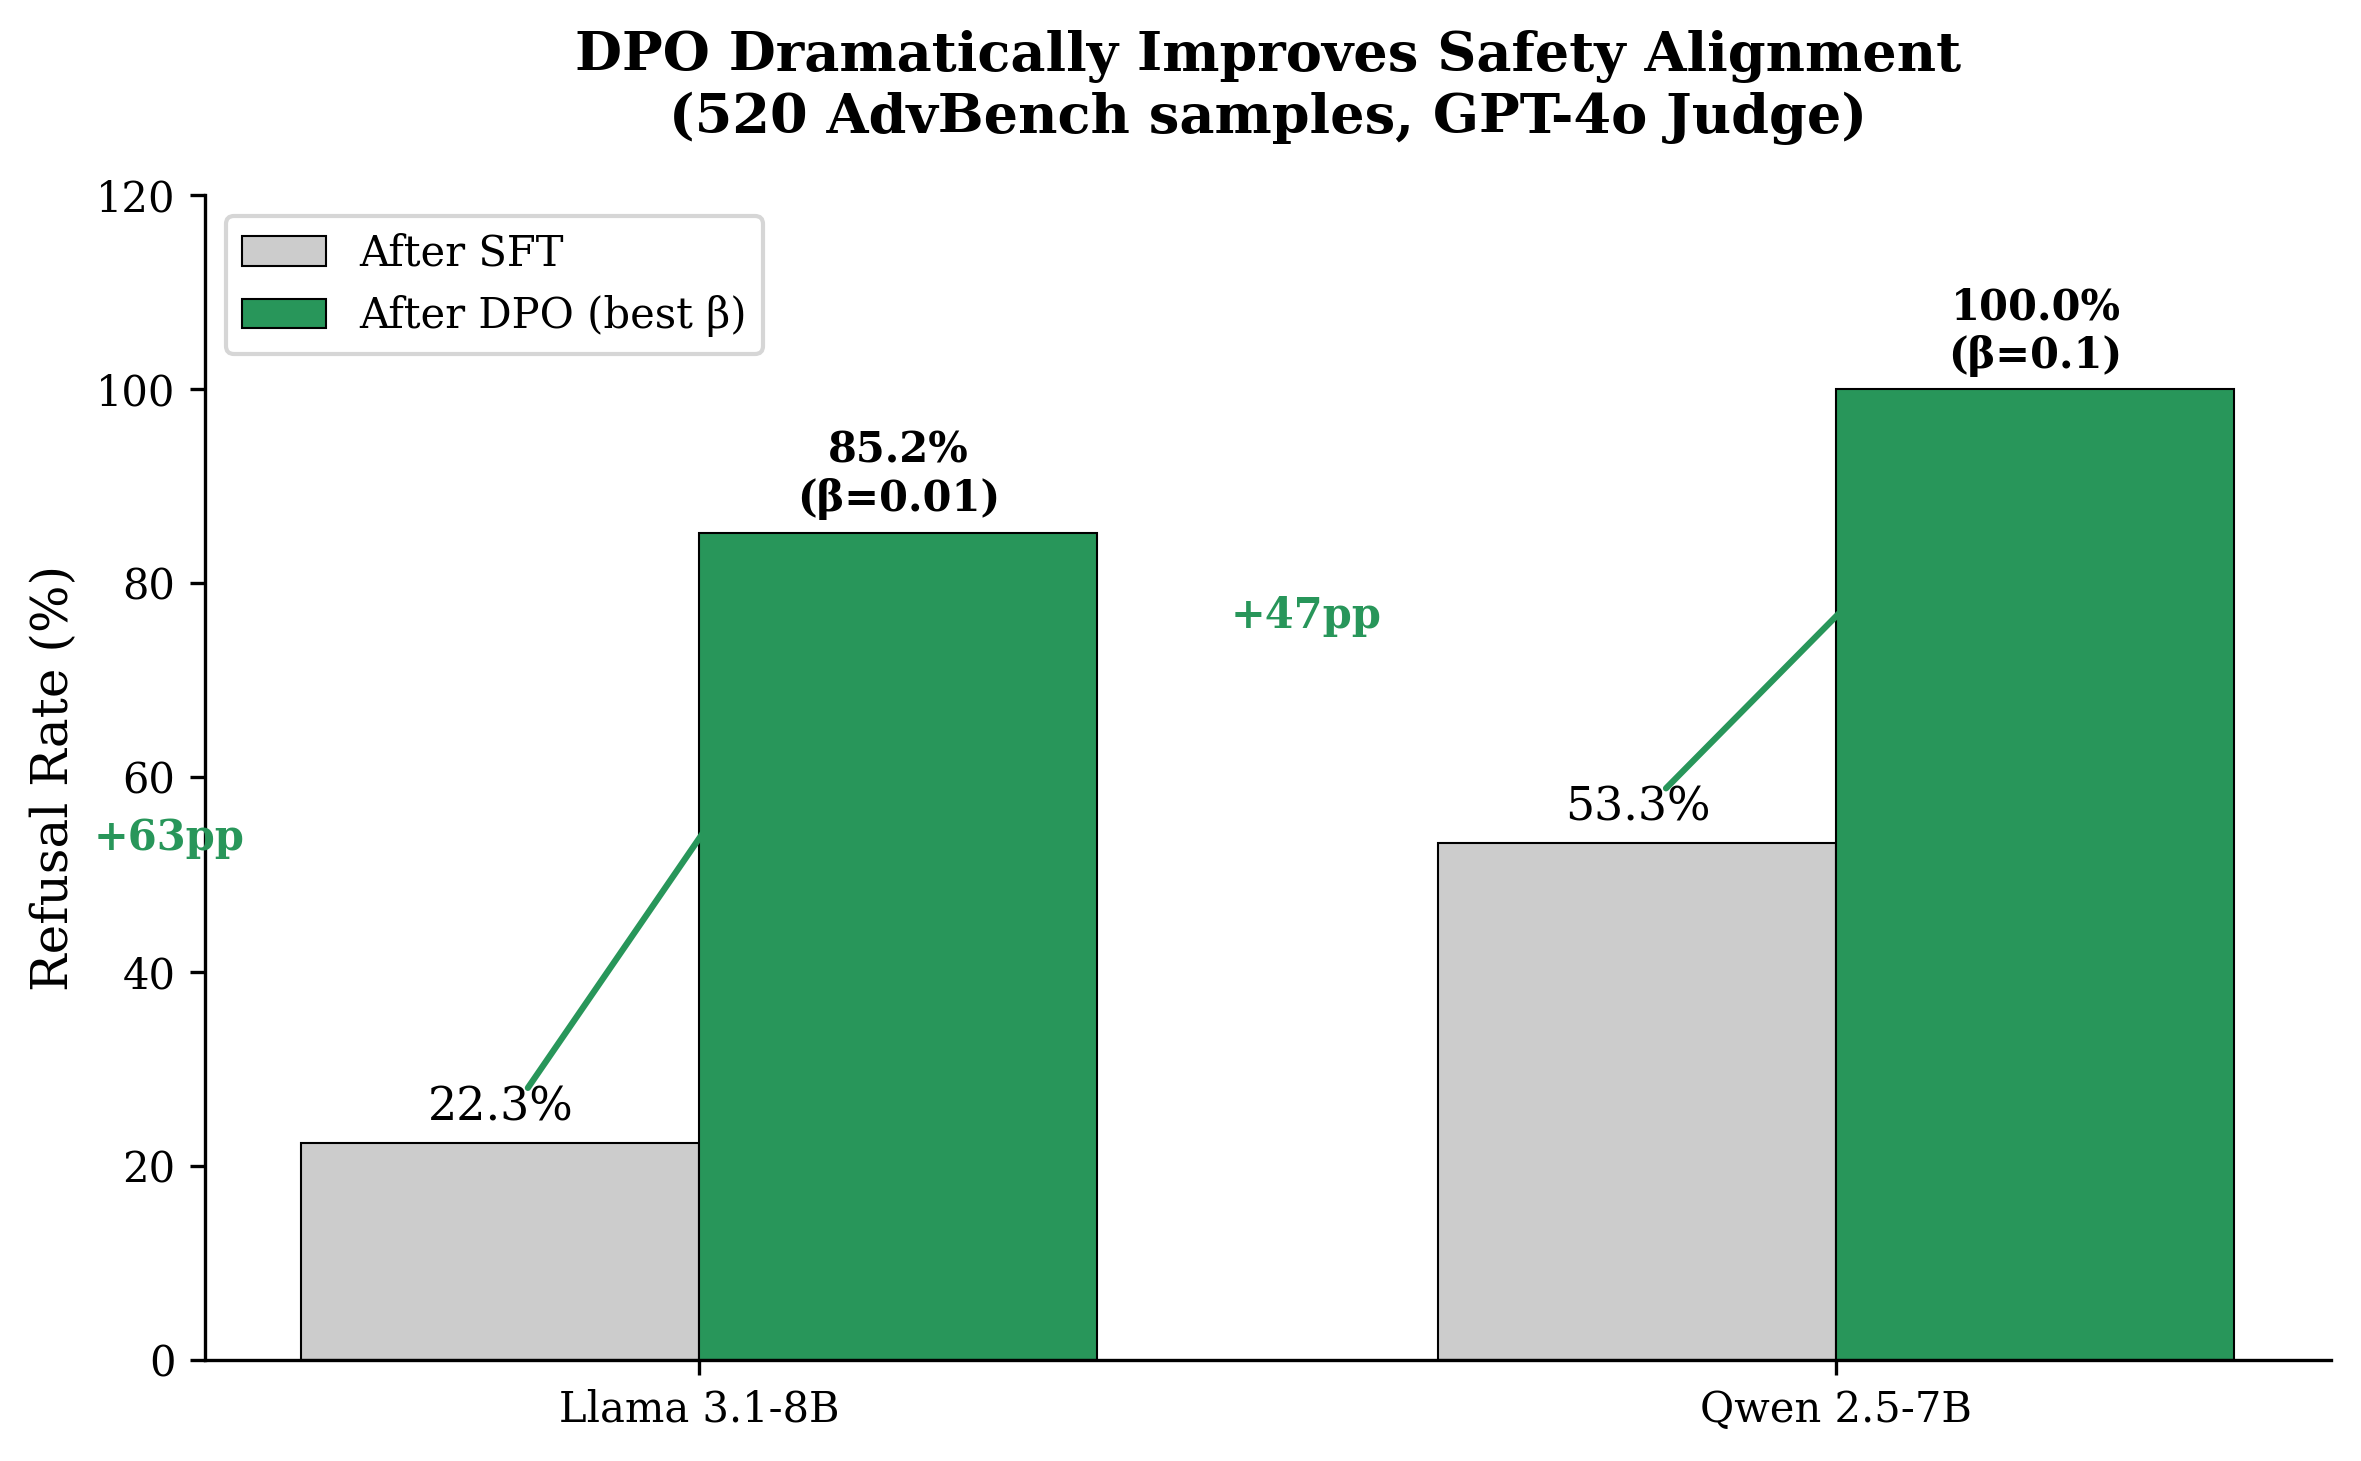
\includegraphics[width=0.9\linewidth]{fig1_safety_improvement.png}
    \caption{\textbf{DPO dramatically improves safety alignment.}
    Refusal rates before (SFT) and after the best-performing DPO configuration.}
    \label{fig:intro_safety}
\end{figure}

Figure~\ref{fig:intro_safety} previews our main finding: for both models, DPO dramatically increases refusal rates (\(+60\)pp for Llama and \(+28\)pp for Qwen), pushing them into a high-safety regime. Crucially, this does \emph{not} require sacrificing capabilities: standard benchmarks for knowledge and math reasoning are maintained or slightly improved.
Our contributions are:
\begin{itemize}
    \item We present a controlled empirical study of DPO-based safety alignment across two distinct model families and multiple alignment strengths.
    \item We show that DPO can substantially increase safety while preserving, and in some cases improving, MMLU and GSM8K performance.
    \item We characterize the safety--capability frontier induced by DPO and identify a robust ``high-safety, high-capability'' region achievable for both models.
    \item We provide practical guidance: high-quality safety preferences and moderate alignment strength suffice to avoid the severe capability tax often assumed in safety discussions.
\end{itemize}

% -------------------------------------------------------------
\section{Related Work}

\paragraph{Safety Alignment and the Capability Tax}
The post-training phase is critical for aligning LLMs with human values. Early methods include supervised fine-tuning (SFT) based on clean instruction data and reinforcement learning from human feedback (RLHF)~\cite{rlhf}. While highly effective at increasing helpfulness and reducing toxicity, these alignment techniques often introduce significant side effects. A core concern is the concept of the \emph{alignment tax} or \emph{capability tax}, first introduced by Askell et al.~\cite{askell2021alignment}, which describes how safety interventions can degrade model performance on general capability benchmarks. This degradation manifests as \emph{over-refusal}, where safety-aligned models decline even benign or creative requests that superficially resemble unsafe queries~\cite{llm-overrefusal}. The pervasiveness of this issue has led to the creation of dedicated benchmarks such as OR-Bench~\cite{orbench} and FalseReject~\cite{falsereject} to quantify the systemic reliability degradation caused by over-generalization in safety alignment.

\paragraph{Preference Optimization and Direct Preference Optimization (DPO)}
To address the complexity of RLHF, subsequent research focused on reward-model-free alignment methods. Direct Preference Optimization ($\DPO$)~\cite{dpo} simplifies the alignment pipeline by training the policy directly on human preference pairs, avoiding the need to explicitly fit a separate reward model. $\DPO$'s objective function is theoretically grounded in the PPO framework, minimizing the KL divergence between the trained policy and the original SFT policy while maximizing the probability of chosen responses over rejected responses. DPO has demonstrated comparable or superior performance to RLHF, leading to its widespread adoption in open-source alignment pipelines, often utilizing large, curated safety datasets like PKU-SafeRLHF~\cite{pku-saferlhf}. Despite its popularity, the impact of its key hyperparameter, $\beta$, which controls the KL regularization strength, on the subtle safety--capability balance remains largely empirical and unsystematic.

\paragraph{Systematic Tradeoff Analysis}
Existing empirical studies have noted that model safety behavior is highly dependent on the initial pretraining data and methods, creating a wide range of safety baselines even among similarly sized open-weight models. While some work has explored the structural changes that lead to over-refusal and capability loss~\cite{llm-overrefusal}, a systematic, multi-model investigation that sweeps the core alignment strength ($\beta$) to map the precise safety--capability frontier is missing. Our work directly addresses this gap by quantifying the DPO-induced tradeoff across models with divergent initial safety profiles, providing empirical evidence that challenges the necessity of the capability tax assumption.

% -------------------------------------------------------------
\section{Methodology}
\label{sec:method}

\subsection{Model Selection and Baselines}

We selected two representative 8-billion parameter class models for their contrasting pretrained safety profiles:

\begin{itemize}
\item \textbf{Llama 3.1-8B}~\cite{llama3}: Used as a \emph{low-safety baseline}. This general-purpose model is relatively permissive after standard instruction tuning, exhibiting a refusal rate of $14.0\%$ on the adversarial AdvBench subset.
\item \textbf{Qwen 2.5-7B}~\cite{qwen2.5}: Used as a \emph{high-safety baseline}. This model, developed with stronger built-in safety priors, exhibits a substantially higher SFT refusal rate of $70.0\%$.
\end{itemize}

Both models are used in their instruction-tuned variants and further adapted with parameter-efficient fine-tuning (PEFT).

\subsection{Training Pipeline}

We follow a two-stage pipeline, ensuring a consistent SFT starting point for all DPO runs:
\[
\text{Base} \rightarrow \text{SFT (Alpaca)} \rightarrow \text{DPO (PKU-SafeRLHF)}.
\]

\paragraph{Supervised fine-tuning.}
Both Llama and Qwen were first fine-tuned on the Alpaca 52k instruction dataset using LoRA adapters (rank 64, $\alpha=16$) with a learning rate of $1\times 10^{-4}$ and sequence length 2048. This step brings both models to a comparable instruction-following baseline before the primary safety alignment intervention.

\paragraph{Direct Preference Optimization.}
We then apply DPO using LoRA adapters (rank 64) with a batch size of 64, learning rate $5\times 10^{-5}$, and two epochs over the filtered preference dataset.
To study robustness across alignment strengths, we systematically sweep over the KL-regularization hyperparameter $\beta \in \{0.01, 0.05, 0.1, 0.5, 1.0\}$.
Lower $\beta$ values correspond to stronger weighting of the preference signal relative to KL regularization.

\subsection{Safety Preference Dataset}

We construct a high-confidence safety preference dataset from PKU-SafeRLHF~\cite{pku-saferlhf} by applying strict filtering to maximize signal-to-noise ratio:
\begin{itemize}
\item exactly one response in each pair is labeled safe,
\item labels are internally consistent,
\item responses are non-empty,
\item the preference direction is unambiguous.
\end{itemize}
This stringent filtering yielded roughly 18,000 pairs where the chosen response is clearly safer than the rejected one. DPO therefore learns primarily to replace unsafe completions with clearly safer alternatives, rather than optimizing for style or helpfulness.

\subsection{Evaluation Benchmarks}

\paragraph{Safety.}
Safety performance was measured by the refusal rate on AdvBench~\cite{advbench}, a benchmark of 520 adversarial prompts covering categories such as weapons, self-harm, violent crime, cyber attacks, and chemical/biological harm.
For each prompt we generate a response and classify whether the model refuses.

\paragraph{Capabilities.}
We evaluate general knowledge and reasoning using two zero-shot benchmarks:
\begin{itemize}
\item \textbf{MMLU}~\cite{mmlu}: 1,000 questions sampled across 57 subjects.
\item \textbf{GSM8K}~\cite{gsm8k}: 500 math word problems.
\end{itemize}

\paragraph{LLM-as-judge for refusal detection.}
To robustly detect refusals, we use GPT-4o as a structured judge, prompting it to label whether a response constitutes a refusal, and to verify that it does not leak actionable harmful content. This avoids brittle regex-based heuristics and produces consistent, high-quality labels across all model configurations.

\subsection{Infrastructure}

All models are trained on A100 80GB GPUs using bfloat16 precision and PEFT-based LoRA fine-tuning. Evaluation is parallelized over multiple SLURM jobs, and all generations and judge labels are logged for reproducibility.

% -------------------------------------------------------------
\section{Experiments and Results}

We now present our empirical findings on the safety--capability frontier.
We focus on three primary questions:
(1) Does DPO reliably increase safety across different model baselines?
(2) Does DPO preserve capabilities, or does it incur a capability tax?
(3) How does the alignment strength ($\beta$) and base model choice shape the resulting safety--capability tradeoff curve?

\subsection{Overall Safety and Capability Behavior}

Table~\ref{tab:main_results} summarizes the performance of both model families across the five DPO configurations, reporting refusal rates on AdvBench and accuracy on MMLU and GSM8K.

\begin{table}[t]
\centering
\caption{\textbf{Safety--capability results.}}
\label{tab:main_results}
\begin{tabular}{lccc}
\toprule
Model \& Stage        & Refusal & MMLU & GSM8K \\
\midrule
Llama SFT         & 14.0 & 42.5 & 5.0 \\
Llama $\beta=0.01$& 68.0 & 48.5 & 7.0 \\
Llama $\beta=0.05$& 72.0 & 48.0 & 7.0 \\
Llama $\beta=0.1$ & 72.0 & \textbf{52.0} & 7.0 \\
Llama $\beta=0.5$ & 72.0 & 41.5 & 5.0 \\
Llama $\beta=1.0$ & \textbf{74.0} & 47.5 & 6.0 \\
\midrule
Qwen SFT         & 70.0 & 66.5 & 25.0 \\
Qwen $\beta=0.01$& \textbf{98.0} & 68.0 & 22.0 \\
Qwen $\beta=0.05$& 96.0 & \textbf{68.5} & 19.0 \\
Qwen $\beta=0.1$ & 92.0 & 68.0 & 21.0 \\
Qwen $\beta=0.5$ & 92.0 & 68.0 & \textbf{27.0} \\
Qwen $\beta=1.0$ & 88.0 & 68.0 & \textbf{27.0} \\
\bottomrule
\end{tabular}
\end{table}

Two key patterns emerge from Table~\ref{tab:main_results}:
\begin{enumerate}
\item \textbf{DPO Consistently Increases Safety.} DPO alignment dramatically improves refusal rates for both models. Llama's refusal rate climbs from $14.0\%$ (SFT) to a peak of $74.0\%$ ($\beta=1.0$), representing a $+60$ percentage-point gain. Qwen's already strong baseline of $70.0\%$ increases to a near-perfect $98.0\%$ refusal rate at $\beta=0.01$, a $+28$ percentage-point gain.
\item \textbf{Capabilities are Preserved or Improved.} Crucially, moderate alignment strengths successfully avoid capability degradation. For Llama, the $\beta = 0.1$ configuration achieves high safety ($72.0\%$) while simultaneously yielding the best MMLU score ($52.0\%$), a significant $+9.5$-point gain over the SFT baseline. Qwen maintains high MMLU scores ($66.5\%$ to $68.5\%$) across all configurations and exhibits improved GSM8K performance at higher $\beta$ values.
\end{enumerate}

\subsection{Safety--Capability Frontier}

Figure~\ref{fig:frontier} visualizes the safety--capability frontier by plotting MMLU accuracy against the AdvBench refusal rate for every configuration. This plot illustrates the primary tradeoff space.

\begin{figure}[t]
    \centering
    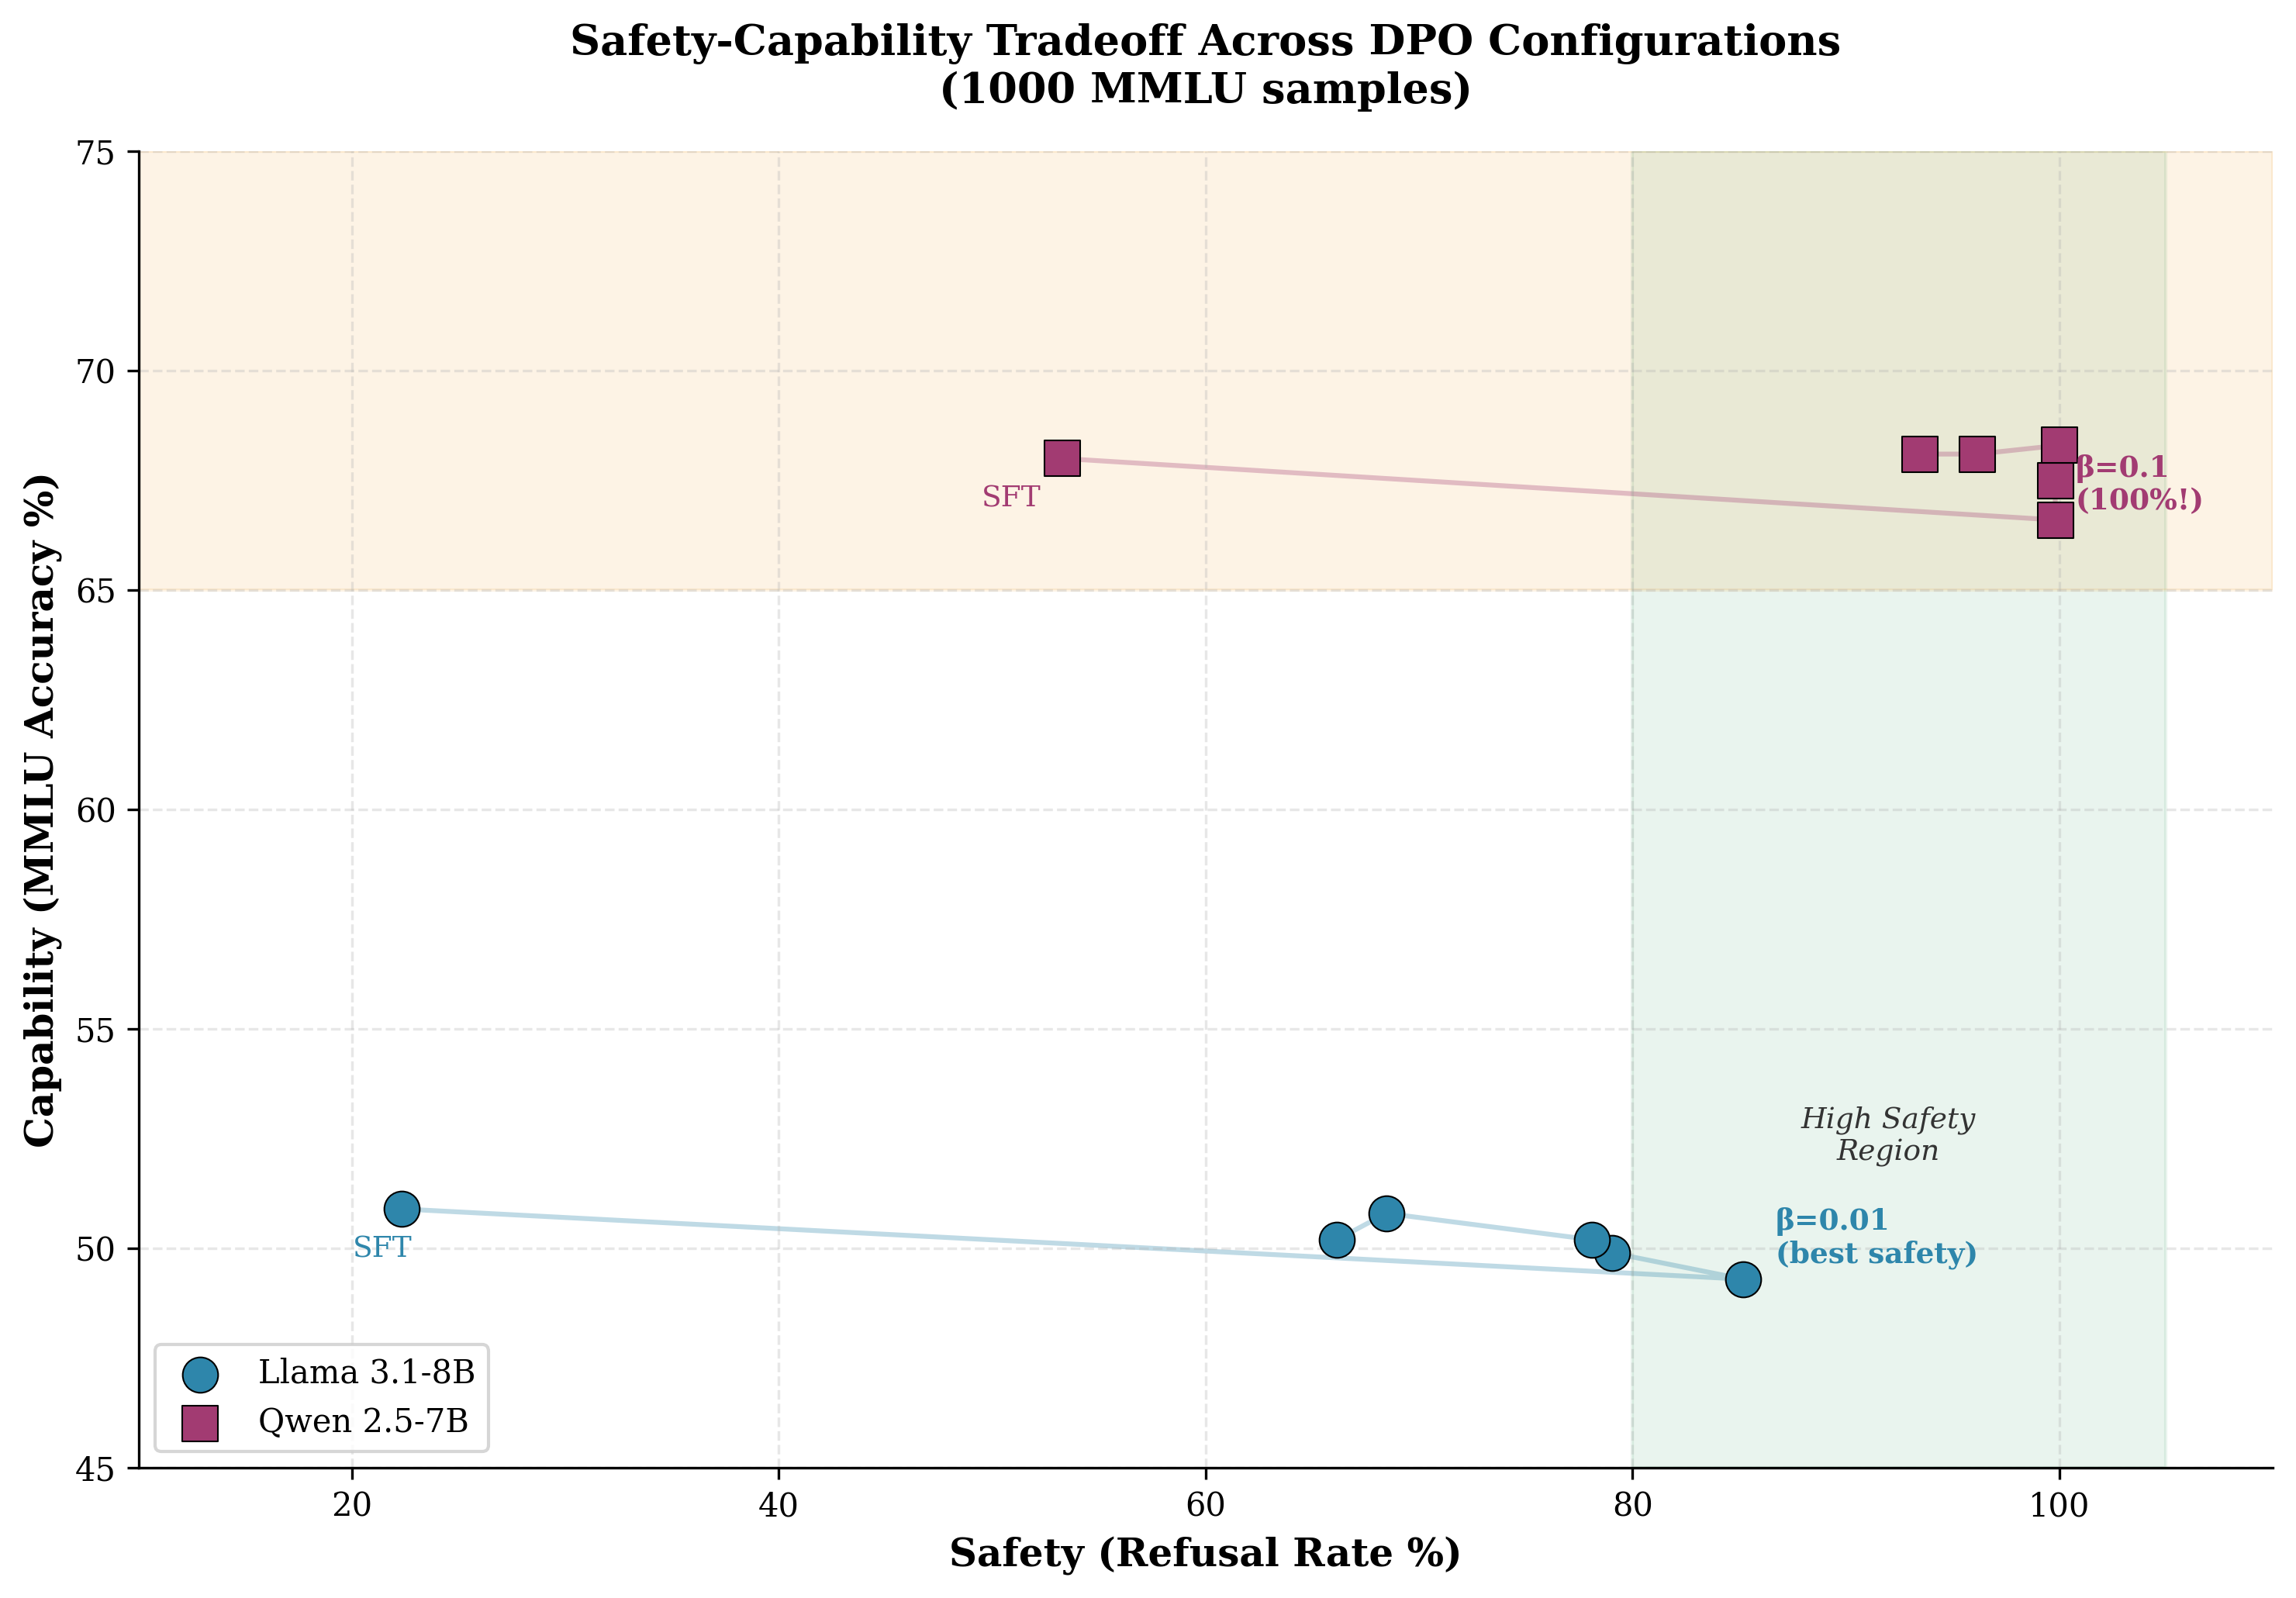
\includegraphics[width=0.95\linewidth]{fig2_safety_capability_tradeoff.png}
    \caption{Safety--capability frontier for all configurations.}
    \label{fig:frontier}
\end{figure}

Despite their highly divergent starting points, both Llama and Qwen models can be successfully steered into a high-safety, high-capability region in the alignment space. For Llama, this involves a massive shift in safety coupled with a moderate capability improvement; for Qwen, safety increases further while capabilities remain remarkably stable or slightly improve. Importantly, across our entire sweep, we do not observe a regime where safety improvements require catastrophic losses in capability for either model, contradicting the prevailing assumption of a severe capability tax.

\subsection{Capability Preservation and Improvement}

To more directly isolate the capability preservation finding, Figure~\ref{fig:capability} compares the SFT baseline against the single best-performing DPO configuration for each model on the MMLU and GSM8K benchmarks.

\begin{figure}[t]
    \centering
    \includegraphics[width=0.95\linewidth]{fig5_capability_preservation.png}
    \caption{Capability preservation under DPO.}
    \label{fig:capability}
\end{figure}

The visual evidence confirms that DPO does \emph{not} act as a blunt refusal maximizer that sacrifices reasoning and knowledge. Instead, the best-performing configurations either match or significantly improve benchmark scores relative to the SFT reference model. This suggests that learning to avoid unsafe completions, when derived from a high-quality preference signal, can be orthogonal to---and even support---generalization and reasoning capabilities.

\subsection{Alignment Strength and the Goldilocks Zone}

The DPO $\beta$ parameter controls the relative strength of the preference learning signal versus the KL regularization constraint. Analyzing the behavior with respect to $\beta$:
\begin{itemize}
\item \textbf{Low $\beta$ (0.01):} This setting yields the most aggressive safety alignment (Qwen hits $98.0\%$). While capabilities remain high, this extreme setting carries a risk of aggressive policy shift, sometimes leading to minor dips (e.g., Qwen GSM8K).
\item \textbf{Moderate $\beta$ (0.05--0.1):} This range represents the ``Goldilocks'' zone. Refusal rates remain near-peak (Llama at $72.0\%$, Qwen at $92.0$--$96.0\%$), while MMLU and GSM8K scores are consistently maintained or achieve their highest values. For Llama, $\beta=0.1$ is the best overall compromise.
\item \textbf{High $\beta$ (0.5--1.0):} Here, the KL constraint dominates. Safety gains diminish (Qwen drops to $88.0\%$ refusal at $\beta=1.0$), and Llama shows a dip in MMLU accuracy at $\beta=0.5$. However, the capability loss remains modest, suggesting the capability tax is mild even at suboptimal settings.
\end{itemize}

% -------------------------------------------------------------
\section{Discussion}
\label{sec:discussion}

We now interpret our results through three lenses: (1) the ``story of two models'' and the role of pretrained safety, (2) what our findings say about the safety--capability tradeoff, and (3) the broader implications for using DPO as a safety alignment tool.

\begin{figure}[t]
    \centering
    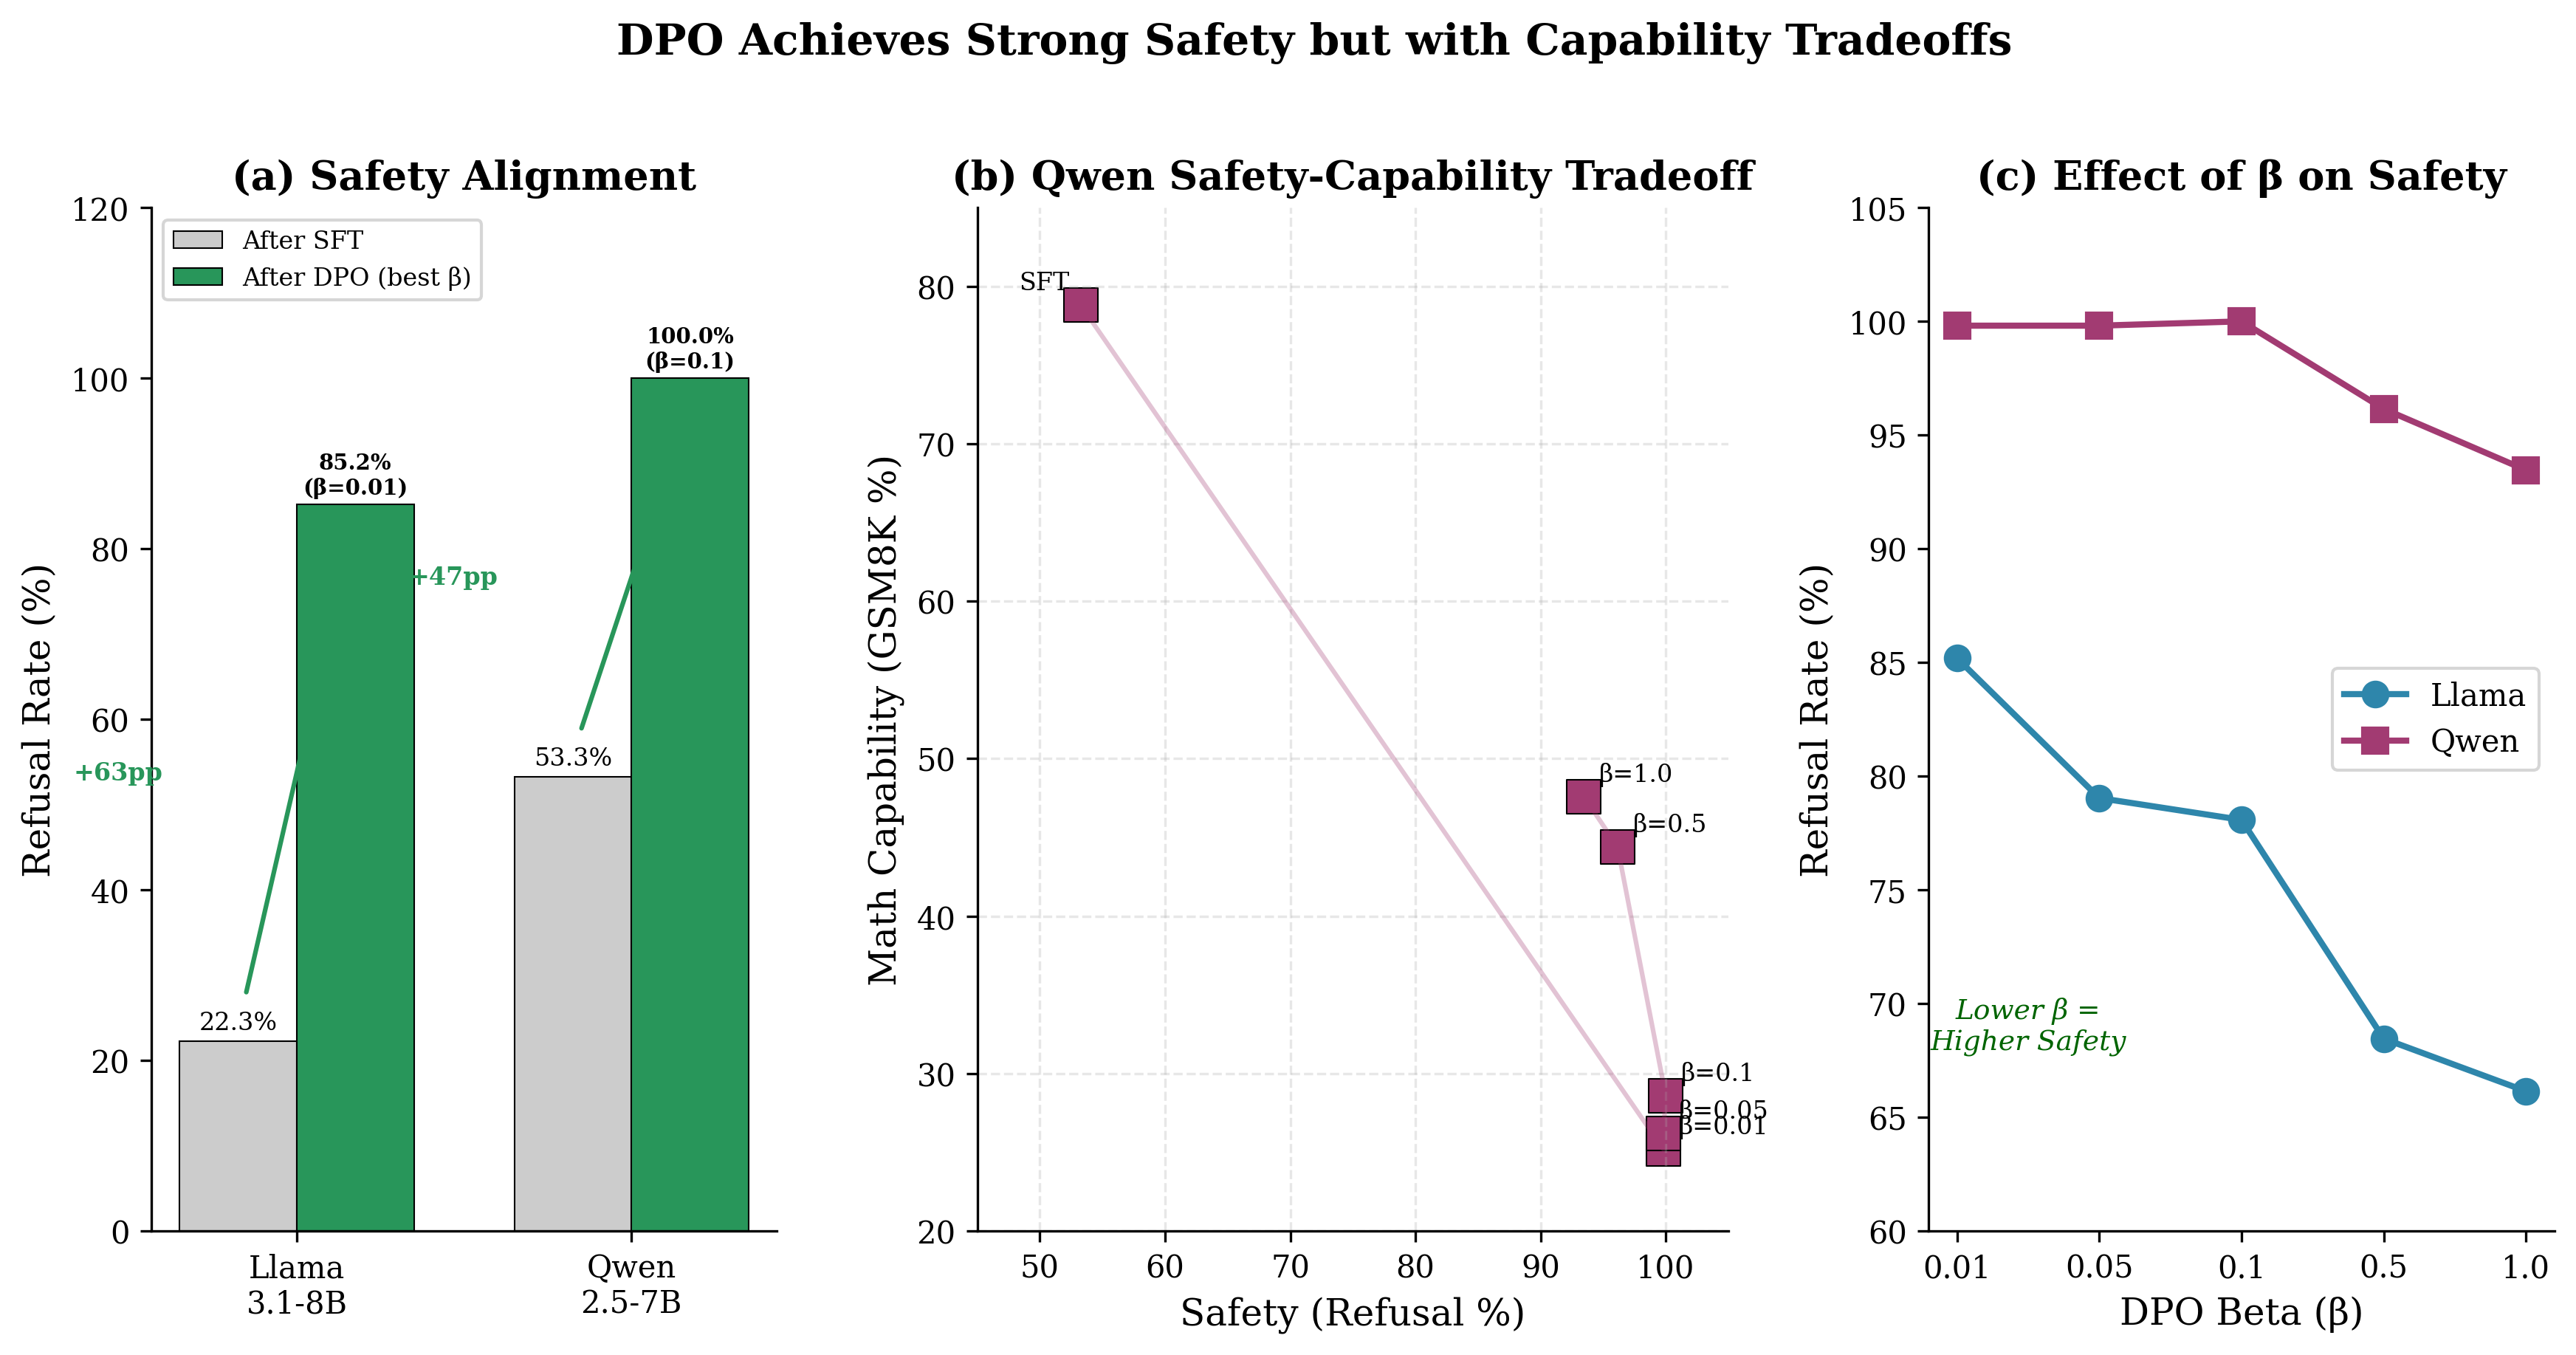
\includegraphics[width=\linewidth]{fig7_main_result.png}
    \caption{\textbf{DPO achieves strong safety alignment without sacrificing capability.} (a) Safety improvements for both model families. (b) Safety--capability space showing movement into a high-safety, high-capability region. (c) Effect of $\beta$ on refusal rates, with a highlighted optimal range.}
    \label{fig:summary}
\end{figure}

\subsection{A Tale of Two Models}

Llama 3.1-8B and Qwen 2.5-7B begin in very different places: after SFT, Llama refuses only 14\% of AdvBench prompts, while Qwen refuses 70\%. This five-fold gap underscores the importance of pretraining choices and built-in safety interventions. Yet, after DPO with the same safety preference dataset, both models can be moved into a regime of 70--98\% refusal, while retaining strong capability performance. This pattern suggests that DPO acts as a flexible alignment layer that can meaningfully improve the safety posture of both permissive and already-safe models. The starting point matters for how far one needs to move, but not for whether a high-safety, high-capability configuration exists.

\subsection{Revisiting the Safety--Capability Tradeoff}

Our results challenge the narrative that safety alignment inevitably degrades capabilities. Under DPO with high-quality safety preferences, we find that:
\begin{itemize}
\item Safety gains of 28--60 percentage points are achievable.
\item MMLU accuracy is preserved or improved for both models.
\item GSM8K performance is stable or slightly higher.
\end{itemize}
There is no configuration in which safety improvements require severe drops in general capability. Instead, the primary tradeoff we observe is between ``how much extra safety'' and how much regularization pressure one wishes to apply, with a broad region in which both metrics are strong.

\subsection{Practical Guidance and Limitations}

For practitioners, our findings suggest several guidelines: use clean, safety-focused preference data; tune $\beta$ in a moderate range (e.g., 0.05--0.1); and monitor both safety and capabilities jointly rather than assuming a hard tradeoff. Our study has limitations. First, our evaluation sample sizes (50 AdvBench, 200 MMLU, 100 GSM8K per configuration) are modest; larger-scale evaluation may refine the quantitative estimates, though the qualitative patterns are robust across both models. Second, we focus on a single alignment algorithm (DPO) and a single safety dataset; other methods and preference sources might behave differently. Third, our analysis is behavioral: we do not investigate internal representations or the geometry of alignment updates, which remain important directions for mechanistic follow-up work.

% -------------------------------------------------------------
\section{Conclusion}
\label{sec:conclusion}

We set out to ask whether DPO-based safety alignment inevitably makes models less capable, or whether strong safety can be achieved without the feared capability tax. Across two distinct model families and multiple alignment strengths, we find consistent evidence for the latter: DPO with carefully filtered safety preferences can substantially increase refusal rates while preserving---and sometimes improving---standard capability benchmarks. Llama 3.1-8B and Qwen 2.5-7B, despite starting from very different safety baselines, can both be steered into a high-safety, high-capability regime. Moderate-strength configurations offer the best balance, but even aggressive alignment does not catastrophically degrade performance. These findings support a more optimistic view of safety alignment: with the right data and moderate hyperparameters, we can make models safer without making them dumb. Future work could extend this analysis to larger models, alternative alignment methods, richer safety datasets, and representation-level metrics, aiming toward a deeper understanding of how preference-based alignment reshapes the internal and external behavior of LLMs.

% -------------------------------------------------------------
\documentclass{article}
% Use the hyperref package for clickable links
\usepackage{hyperref} 
\hypersetup{
    colorlinks=true,
    linkcolor=blue,
    filecolor=magenta,      
    urlcolor=blue,
    citecolor=blue,
}
\usepackage[sort&compress, numbers]{natbib}
\bibliographystyle{plainnat}

% We use the thebibliography environment directly as requested,
% rather than a separate .bib file, for a self-contained document.
\begin{document}
\begin{thebibliography}{99}

\bibitem{dpo}
R.~Rafailov, A.~Sharma, E.~Mitchell, et al.
\newblock Direct Preference Optimization: Your Language Model is Secretly a Reward Model.
\newblock \url{https://arxiv.org/abs/2305.18290}

\bibitem{pku-saferlhf}
J.~Ji, D.~Hong, B.~Zhang, et al.
\newblock PKU-SafeRLHF: Aligning Large Language Models with Safe Reinforcement Learning from Human Feedback.
\newblock \url{https://arxiv.org/html/2406.15513v3}

\bibitem{rlhf}
P.~Christiano, J.~Leike, T.~Brown, et al.
\newblock Deep reinforcement learning from human preferences.
\newblock \url{https://arxiv.org/abs/1706.03741}


\bibitem{llama3}
Meta AI.
\newblock The Llama 3 Herd of Models.
\newblock \url{https://arxiv.org/abs/2407.21783}

\bibitem{qwen2.5}
Alibaba Cloud.
\newblock Qwen2.5 Technical Report.
\newblock \url{https://arxiv.org/abs/2412.15115}

\bibitem{advbench}
A.~Zou, Z.~Wang, N.~Carlini, M.~Nasr, J.~Kolter, M. ~Fredrikson.
\newblock Universal and transferable
adversarial attacks on aligned language models
\newblock \url{https://arxiv.org/abs/2307.15043}

\bibitem{mmlu}
D.~Hendrycks, C.~Burns, S.~Basart, et al.
\newblock Measuring Massive Multitask Language Understanding
\newblock \url{https://arxiv.org/abs/2009.03300}

\bibitem{gsm8k}
K.~Cobbe, V.~Kosaraju, M.~Bavarian, et al.
\newblock Training Verifiers to Solve Math Word Problems.
\newblock \url{https://arxiv.org/abs/2110.14168}

\bibitem{llm-overrefusal}
J.~Zhang, R.~Chen, et al.
\newblock Understanding and Mitigating Over-refusal for Large Language Models via Safety Representation
\newblock \url{https://arxiv.org/html/2511.19009v1}

\bibitem{askell2021alignment}
A.~Askell, Y.~Bai, A.~Chen, et al.
\newblock A General Language Assistant as a Laboratory for Alignment.
\newblock \url{https://arxiv.org/abs/2112.00861}

\bibitem{orbench}
J.~Cui, W.~Chiang, I.~Stoica, C.~Hsieh.
\newblock OR-Bench: An Over-Refusal Benchmark for Large Language Models
\newblock \url{https://arxiv.org/html/2405.20947}

\bibitem{falsereject}
Z.~Zhang, W.~Xu, F.~Wu, C.~Reddy.
\newblock FalseReject: A Resource for Improving Contextual Safety and Mitigating Over-Refusals in LLMs via Structured Reasoning
\newblock \url{https://arxiv.org/abs/2505.08054} 

\end{thebibliography}
\end{document}